% Presentación demo — Caso técnico Rappi (Módulos 1, 2 y 3)
% Estructura: Problema → Métrica → Diagnóstico (M1) → Insight → Acción → Limitaciones → Extensión → observabilidad → cierre.
% Compilar: pdflatex presentacion_demo.tex (dos veces para TOC)
\documentclass[aspectratio=169,spanish]{beamer}

\usepackage[utf8]{inputenc}
\usepackage[T1]{fontenc}
\usepackage[spanish]{babel}
\usepackage{graphicx}
\usepackage{booktabs}
\usepackage{array}
\usepackage{xcolor}
\usepackage{tikz}
\usetikzlibrary{arrows.meta,positioning,fit,calc}

\usetheme{Madrid}
\usecolortheme{default}

\definecolor{rappiaccent}{HTML}{9B2222}
\setbeamercolor{structure}{fg=rappiaccent}
\setbeamercolor{palette primary}{fg=white,bg=rappiaccent}
\setbeamercolor{palette secondary}{fg=white,bg=rappiaccent!85!black}
\setbeamercolor{frametitle}{fg=white,bg=rappiaccent}
\setbeamercolor{title}{fg=white}
\setbeamercolor{subtitle}{fg=white!92}
\setbeamertemplate{navigation symbols}{}
% Numeración: diapositiva actual / total (misma convención que Beamer para handout).
\setbeamertemplate{footline}{%
  \leavevmode%
  \hbox{%
    \begin{beamercolorbox}[wd=\paperwidth,ht=2.5ex,dp=1ex,leftskip=1em,rightskip=1em]{author in head/foot}%
      \usebeamerfont{author in head/foot}%
      \usebeamercolor[fg]{author in head/foot}%
      \hfill\insertframenumber\,/\,\inserttotalframenumber
    \end{beamercolorbox}%
  }%
}

\newenvironment{piegrafica}{%
  \par\vspace{0.5em}%
  \noindent
  \begin{minipage}[t]{\linewidth}%
  \raggedright
  \setlength{\parindent}{0pt}%
  \setlength{\parskip}{0.42em plus 0.12em minus 0.06em}%
  \scriptsize
}{%
  \end{minipage}\par
}

\newenvironment{piegraficafoot}{%
  \par\vspace{0.5em}%
  \noindent
  \begin{minipage}[t]{\linewidth}%
  \raggedright
  \setlength{\parindent}{0pt}%
  \setlength{\parskip}{0.42em plus 0.12em minus 0.06em}%
  \footnotesize
}{%
  \end{minipage}\par
}

\newcommand{\pizoneread}{%
  \begin{piegrafica}
  Frecuencia por hora del \texttt{ratio} en \emph{esta} zona (histórico del panel).

  Complementa los gráficos P1 agregados y muestra en qué franjas aparecen colas o picos.
  \end{piegrafica}%
}

\title[Sistema de alertas]{Alertas cuando llueve y la operación intensifica.}
\subtitle{Caso Rappi · Datos + reglas por zona + mensaje en Telegram}
\author{Demo técnica}
\date{\today}

\begin{document}

\begin{frame}
  \titlepage
\end{frame}

\begin{frame}{Qué vamos a ver}
  \tableofcontents
\end{frame}

% ---------------------------------------------------------------------------
\section{Problema}

\begin{frame}{Rappi pierde eficiencia por desbalance dinámico}
  \begin{itemize}
    \item La \textbf{oferta} (repartidores conectados) y la \textbf{demanda} (pedidos) \emph{no} se equilibran de forma estable: cambian por \textbf{zona}, \textbf{hora} y \textbf{contexto} (clima, día, incentivos).
    \item Ese desbalance se manifiesta en colas, saturación puntual y decisiones tarde: hacen falta \textbf{avisos a tiempo} y \textbf{números concretos} (zona, gravedad, cuánto subir incentivos).
    \item La solución del caso no es un ``modelo mágico'' a ciegas: primero se \textbf{aprende del histórico} (Excel + notebook) y luego el código aplica \textbf{reglas claras} y parámetros versionados (\texttt{calibration.json}).
  \end{itemize}
\end{frame}

\begin{frame}{Tres bloques, una idea cada uno}
  \begin{description}
    \item[Módulo 1] \textbf{Diagnóstico:} con el Excel y el notebook se entiende cómo reacciona cada zona; de ahí salen sensibilidades y umbrales.
    \item[Módulo 2] \textbf{Motor:} mira el \textbf{clima en vivo} (Open-Meteo), aplica las reglas por zona y dice riesgo e incentivos.
    \item[Módulo 3] \textbf{Mensaje:} convierte ese resultado en \textbf{texto para humanos} (modelo de lenguaje o plantilla de respaldo) y lo manda a \textbf{Telegram}.
  \end{description}
\end{frame}

\begin{frame}{Arquitectura del pipeline}
  \centering
  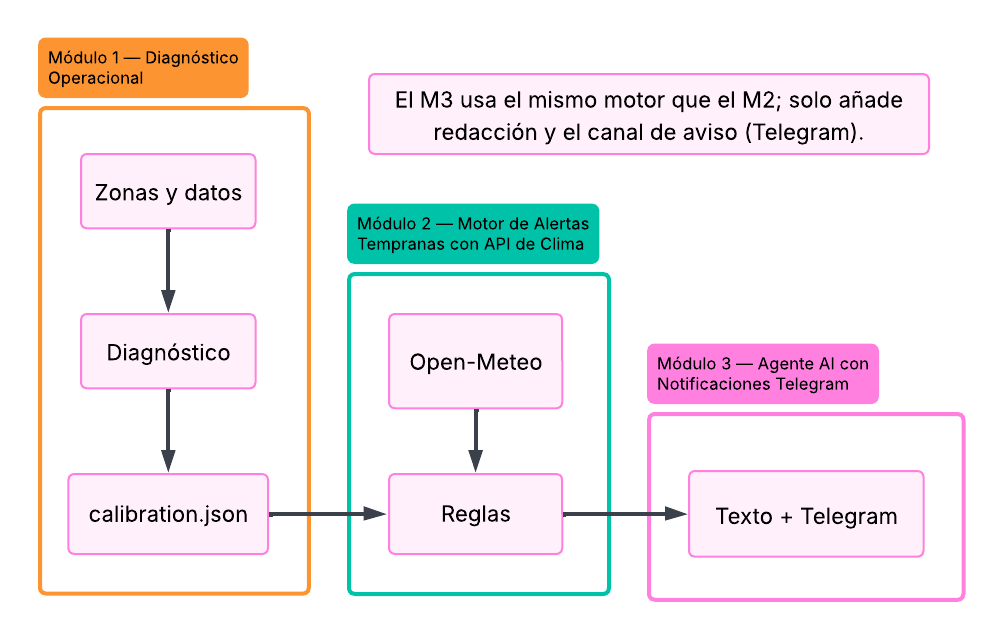
\includegraphics[width=\linewidth,height=0.80\textheight,keepaspectratio]{figures/pipeline_arquitectura.png}

\end{frame}

% ---------------------------------------------------------------------------
\section{Métrica clave: ratio pedidos/repartidor}

\begin{frame}{Qué mide el \texttt{ratio} y cómo se etiqueta el panel}
  \begin{itemize}
    \item \textbf{Definición:} \texttt{ratio} $=$ pedidos entre repartidores conectados en esa celda (zona $\times$ hora); resume el \textbf{apretón} operativo relativo.
    \item \textbf{Saturación:} si el \texttt{ratio} supera \textbf{1{,}8} la celda se trata como saturada en el diagnóstico.
    \item \textbf{Otras bandas:} sobre-oferta si ${<}\,0{,}5$; ``saludable'' entre $0{,}9$ y $1{,}2$; el resto es intermedio.
    \item \textbf{Panel:} 30 días $\times$ 24 h $\times$ 14 zonas $=$ 10\,080 filas en el Excel de referencia.
  \end{itemize}
\end{frame}

% ---------------------------------------------------------------------------
\section{Diagnóstico: zonas y horas críticas}

\begin{frame}{Variables que se utilizan para calibrar el motor}
  \small
  \begin{itemize}
    \item \textbf{\texttt{precip\_coef}} — cuánto sube el ``apretón'' operativo cuando sube un poco la lluvia (estimado como en el notebook).
    \item \textbf{\texttt{sensitivity\_index}} — qué tan ``nerviosa'' es la zona frente a lluvia, comparada con el resto (número entre 0 y 1).
    \item \textbf{\texttt{alert\_precip\_mm\_hr}} — a partir de cuánta lluvia (mm/h) tiene sentido considerar alerta, según el histórico de horas ``malas''.
    \item \textbf{\texttt{mm\_precip\_healthy\_to\_saturation\_linear}} — orden de magnitud de lluvia para pasar de ``normal'' a ``muy cargado'' en esa zona.
    \item \textbf{\texttt{base\_earnings\_mxn}} — mediana histórica de pagos en la zona.
    \item \textbf{\texttt{recommended\_earnings\_mxn}} — media cuando ya llovía por encima del umbral (M1); el motor interpola entre base y recomendado según el ratio proyectado (tope global 35\,\%).
  \end{itemize}
\end{frame}

\begin{frame}{Cosas que el diagnóstico deja en claro}
  \footnotesize
  \begin{enumerate}
    \item El panel tiene \textbf{30 días $\times$ 24 h $\times$ 14 zonas} (10\,080 filas). 
    \item La lluvia \textbf{sí se asocia} con más presión operativa.
    \item Hay una asociación con patrones temporales específicos, en ciertos horarios del día (Comida y Cena).
    \item Se observan incrementos en días festivos, así como en días particulares de la semana como jueves y martes.
    \item Existe una posible influencia de eventos locales, que podrían intensificar la demanda y elevar saturación.
    \item Si en una hora hay más de \textbf{0{,}5 mm/h} de lluvia, la probabilidad de saturación es unas \textbf{8 veces} mayor que con lluvia muy suave o nula.
    \item \textbf{Cada zona es distinta:} por ejemplo Santiago reacciona antes que Mitras.
    \item \textbf{Mapas:} la mayoría de polígonos vienen bien; donde falta, se usan centroides. 
    \item Los resultados deben interpretarse con cautela, ya que pueden estar afectados por variables de confusión.
    \item Es necesario validar si los efectos observados son causales o circunstanciales.
    \item Se recomienda incorporar variables como el tipo de zona (urbana vs. rural).
  \end{enumerate}
  \vspace{0.25em}
  \tiny Más detalle: \texttt{modulo1\_diagnostico/HALLAZGOS\_M1.md}
\end{frame}

% Figuras y tablas M1 (notebook 01_diagnostico_operacional.ipynb) — incluido desde presentacion_demo.tex
% Rutas relativas al directorio demo_caso_tecnico/



\begin{frame}{Clasificación operativa — conteos y \% (sobre filas con etiqueta)}
  \begingroup
  \centering
  \renewcommand{\arraystretch}{1.35}
  {\normalsize
  \begin{tabular}{@{}lrrp{0.52\textwidth}@{}}
    \toprule
    \textbf{\texttt{clasificacion}} & \textbf{$n$ filas} & \textbf{\%} & \textbf{Criterio sobre \texttt{ratio}} \\
    \midrule
    intermedio   & 4807 & 47{,}69 & Resto: $[\,0{,}5,\,0{,}9)$ o $(\,1{,}2,\,1{,}8\,]$. \\
    saludable    & 2503 & 24{,}83 & $0{,}9 \le \texttt{ratio} \le 1{,}2$. \\
    sobre\_oferta & 2257 & 22{,}39 & $\texttt{ratio} < 0{,}5$. \\
    saturacion   & 513  & 5{,}09  & $\texttt{ratio} > 1{,}8$. \\
    \bottomrule
  \end{tabular}
  }
  \par
  \endgroup

  \begin{piegraficafoot}
  La columna \texttt{clasificacion} resume el estado frente a umbrales de \texttt{ratio} del diagnóstico (saludable, saturación, etc.). Los porcentajes son sobre filas con categoría (aquí, las 10\,080 con \texttt{ratio} válido).
  \end{piegraficafoot}

  \begin{piegrafica}
  La mayoría del panel está fuera de saturación; $\approx 5\%$ de celdas superan el umbral operativo. IC95\% Wilson para la proporción global en saturación: $[0{,}0468,\,0{,}0554]$.
  \end{piegrafica}
\end{frame}



\begin{frame}{P1 — Saturación por hora del día}
  \begingroup
  \centering
  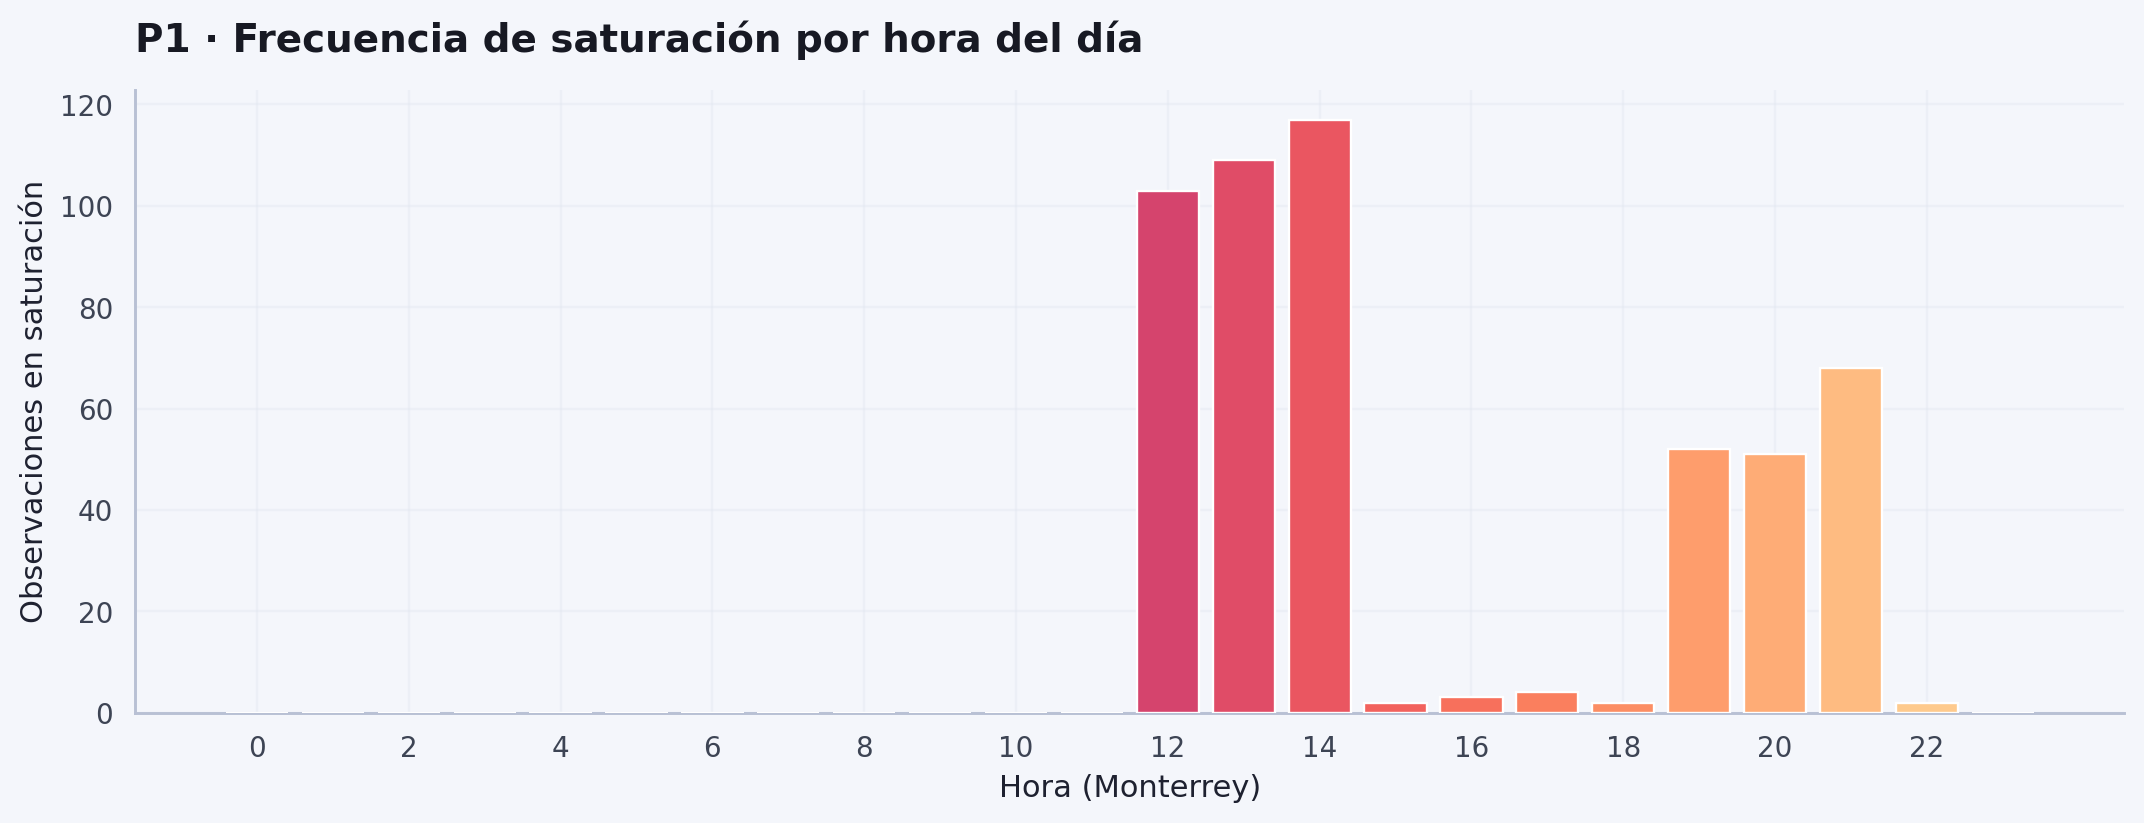
\includegraphics[width=\linewidth,height=0.70\textheight,keepaspectratio]{../modulo1_diagnostico/figures/p1_horas_saturacion.png}
  \par
  \endgroup
  \begin{piegrafica}
  P1 responde \emph{¿a qué horas} aparece más a menudo el ratio por encima del umbral de saturación? No es predicción; es \textbf{conteo} en el historial del Excel.

  El gráfico acumula filas con \texttt{clasificacion}${}=$\texttt{saturacion} (\texttt{ratio}${}>1{,}8$) por hora.
  \end{piegrafica}
\end{frame}

\begin{frame}{P1 — Horas con mayor fracción empírica de saturación}
  \begingroup
  \centering
  \footnotesize
  \renewcommand{\arraystretch}{1.15}
  \begin{tabular}{@{}crr@{}}
    \toprule
    \texttt{HOUR} & $p_{\text{sat}}$ & $n$ \\
    \midrule
    14 & $0{,}2786$ & 420 \\
    13 & $0{,}2595$ & 420 \\
    12 & $0{,}2452$ & 420 \\
    21 & $0{,}1619$ & 420 \\
    19 & $0{,}1238$ & 420 \\
    20 & $0{,}1214$ & 420 \\
    17 & $0{,}0095$ & 420 \\
    16 & $0{,}0071$ & 420 \\
    \bottomrule
  \end{tabular}
  \par
  \endgroup
\end{frame}

\begin{frame}{P1 — Zonas con más celdas en saturación}
  \begingroup
  \centering
  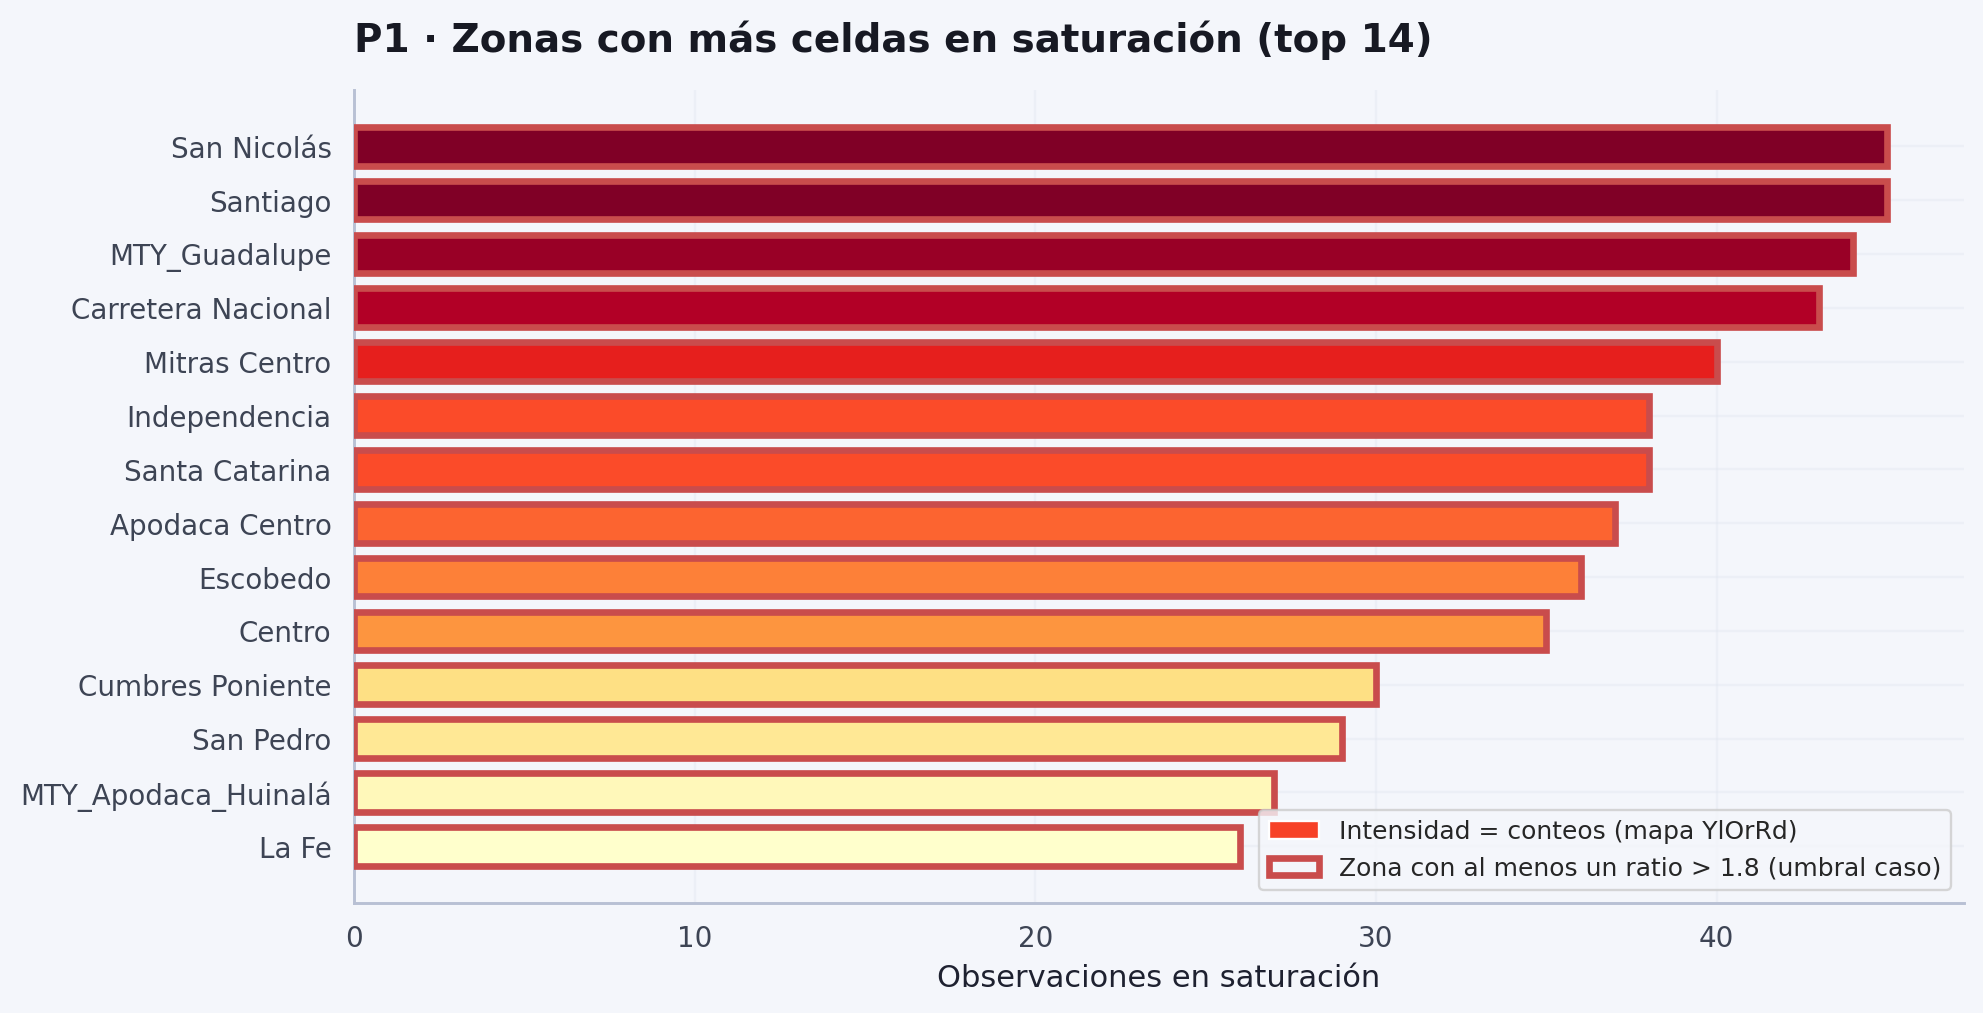
\includegraphics[width=\linewidth,height=0.70\textheight,keepaspectratio]{../modulo1_diagnostico/figures/p1_zonas_saturacion.png}
  \par
  \endgroup
  \begin{piegrafica}
  Ordena territorios por \textbf{frecuencia histórica} de saturación en el mes. Sirve para priorizar dónde mirar primero; no sustituye criterio de zona en vivo.
  \end{piegrafica}
\end{frame}


\begin{frame}[t]{P2 — Correlaciones Pearson y MCO}
  \begingroup
  \footnotesize
  \centering
  \textbf{Matriz de correlación de Pearson}\\[0.35em]
  \resizebox{0.92\linewidth}{!}{%
  \begin{tabular}{@{}lrrr@{}}
    \toprule
    & \texttt{PRECIPITATION\_MM} & \texttt{ratio} & \texttt{EARNINGS} \\
    \midrule
    \texttt{PRECIPITATION\_MM} & 1{,}000000 & 0{,}318902 & 0{,}226029 \\
    \texttt{ratio}             & 0{,}318902 & 1{,}000000 & 0{,}099885 \\
    \texttt{EARNINGS}          & 0{,}226029 & 0{,}099885 & 1{,}000000 \\
    \bottomrule
  \end{tabular}%
  }
  \par
  \endgroup

  \vspace{0.3em}
  \begingroup
  \footnotesize
  \raggedright
  \noindent
  $P(\text{saturación} \mid \text{precip} > 0{,}5) = 0{,}3082$ \quad
  $P(\text{saturación} \mid \text{precip} \le 0{,}5) = 0{,}0377$\\[0.25em]
  \par
  \endgroup
\end{frame}

\begin{frame}{P2 — Lluvia, demanda e interacción (lectura cualitativa)}
  \begingroup
  \centering
  \normalsize
  \renewcommand{\arraystretch}{1.35}
  \begin{tabular}{@{}ll@{}}
    \toprule
    \textbf{Hora} & \textbf{Efecto de lluvia} \\
    \midrule
    Mañana & Bajo impacto \\
    Comida & Medio \\
    Cena & \textcolor{rappiaccent}{\textbf{Muy alto}} \\
    \bottomrule
  \end{tabular}
  \par
  \endgroup

  \begin{piegraficafoot}
  La lluvia se asocia a más saturación \textbf{controlando} por hora y zona, pero el efecto \textbf{no es homogéneo}: se \textbf{intensifica en horas de alta demanda} (interacción operativa--externa).

  La tabla es cualitativa y está alineada con GAP~1 (pendiente marginal por hora).
  \end{piegraficafoot}
\end{frame}


\begin{frame}{Exploración — distribución del \texttt{ratio} por zona}
  \begingroup
  \centering
  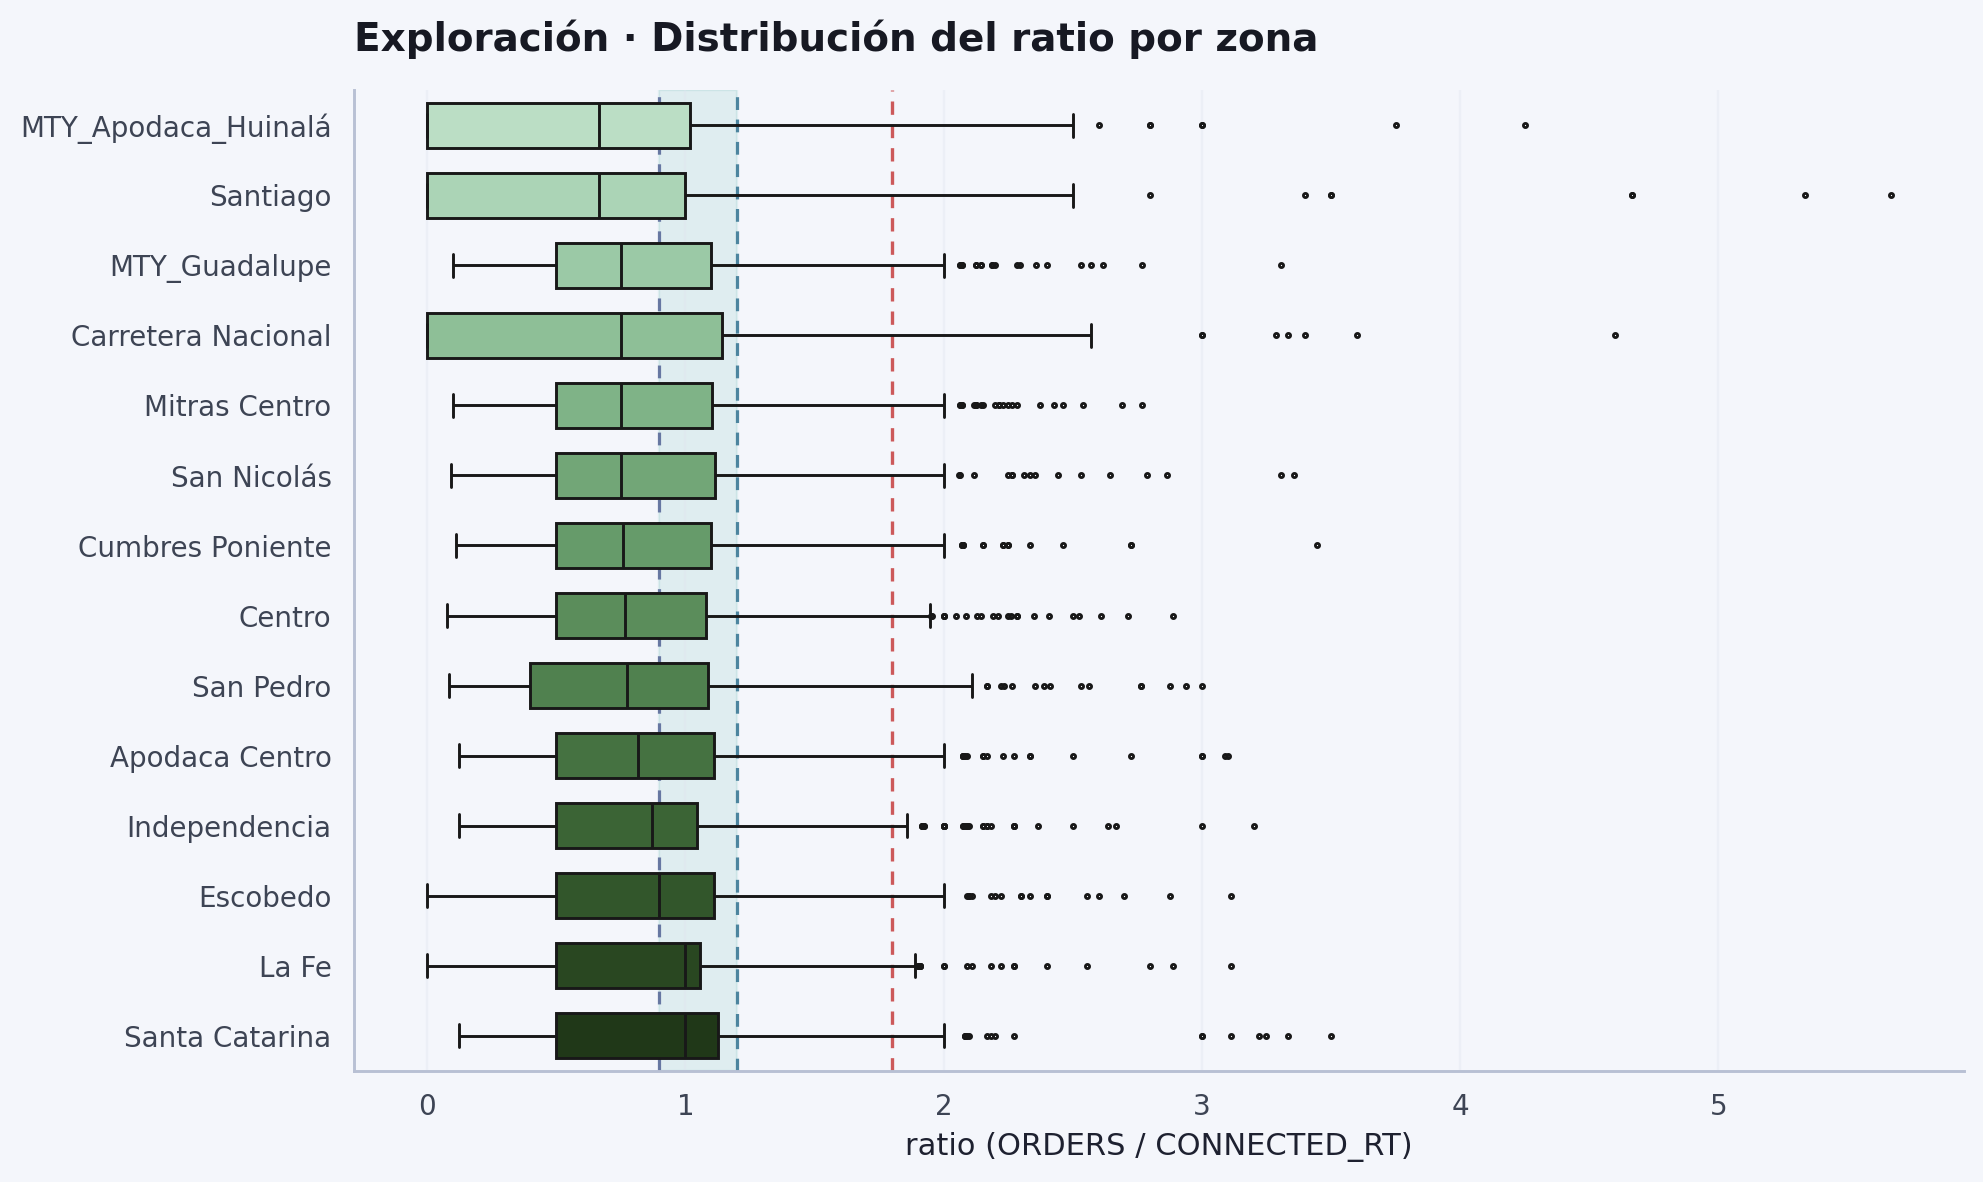
\includegraphics[width=\linewidth,height=0.85\textheight,keepaspectratio]{../modulo1_diagnostico/figures/exploracion_ratio_por_zona.png}
  \par
  \endgroup
\end{frame}


\begin{frame}{GAP 1 — Pendiente marginal de precipitación por hora}
  \begingroup
  \centering
  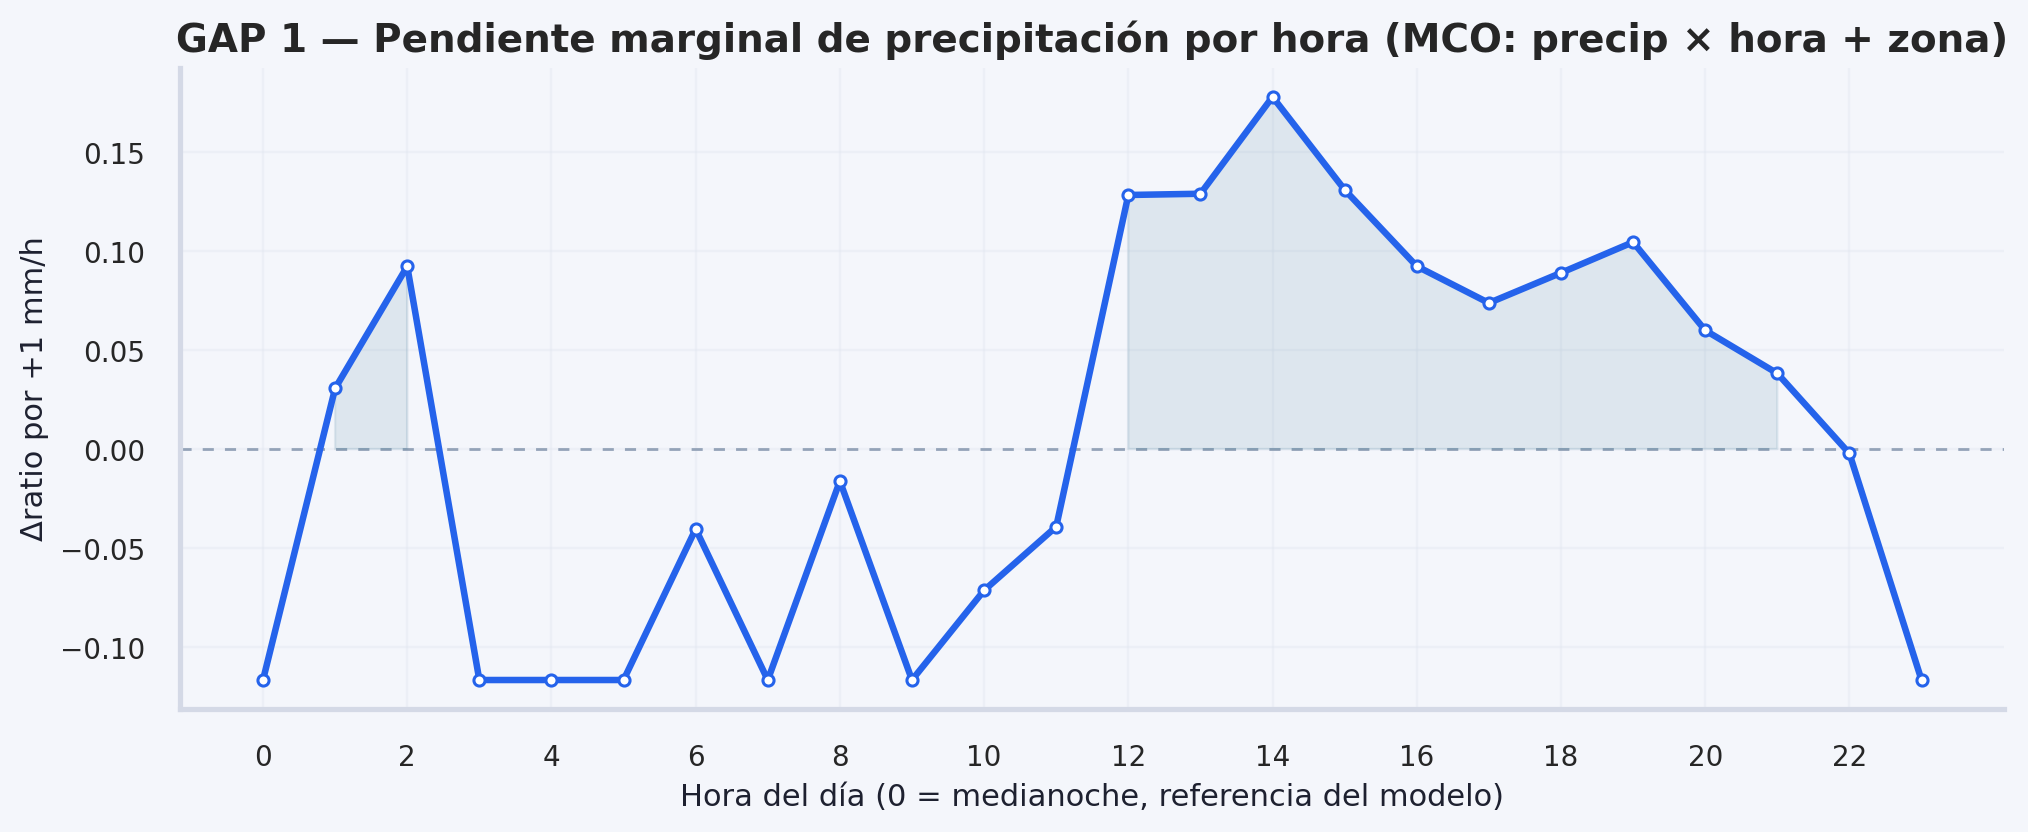
\includegraphics[width=\linewidth,height=0.70\textheight,keepaspectratio]{../modulo1_diagnostico/figures/gap1_precip_marginal_por_hora.png}
  \par
  \endgroup
  \begin{piegrafica}
  Con interacción precipitación$\times$hora, la \textbf{pendiente marginal} de +1~mm/h varía por franja. El gráfico resume $\Delta\text{ratio}$ por hora (referencia \texttt{HOUR}=0).
  \end{piegrafica}
\end{frame}


\begin{frame}{P2b — Tabla: saturación y CV(\texttt{ORDERS}) por tramo de \texttt{ratio}}
  \begingroup
  \footnotesize
  \centering
  \renewcommand{\arraystretch}{1.15}
  \begin{tabular}{@{}lrrr@{}}
    \toprule
    \textbf{Tramo} & $n$ & $p_{\text{saturación}}$ & CV(\texttt{ORDERS}) \\
    \midrule
    $<0{,}9$      & 5780 & $0{,}0000$ & $1{,}1828$ \\
    $0{,}9$--$1{,}2$ & 2422 & $0{,}0000$ & $0{,}7761$ \\
    $1{,}2$--$1{,}5$ &  851 & $0{,}0000$ & $0{,}5082$ \\
    $1{,}5$--$1{,}8$ &  514 & $0{,}0000$ & $0{,}3616$ \\
    $>1{,}8$      &  513 & $1{,}0000$ & $0{,}3685$ \\
    \bottomrule
  \end{tabular}
  \par
  \endgroup

  \begin{piegrafica}
  Proxy de ``estrés'' por bandas de \texttt{ratio}. Solo el tramo $>1{,}8$ coincide con saturación operativa del caso. El CV de pedidos sirve como señal de inestabilidad.
  \end{piegrafica}
\end{frame}

\begin{frame}{P2b — Estrés por tramo de \texttt{ratio}}
  \begingroup
  \centering
  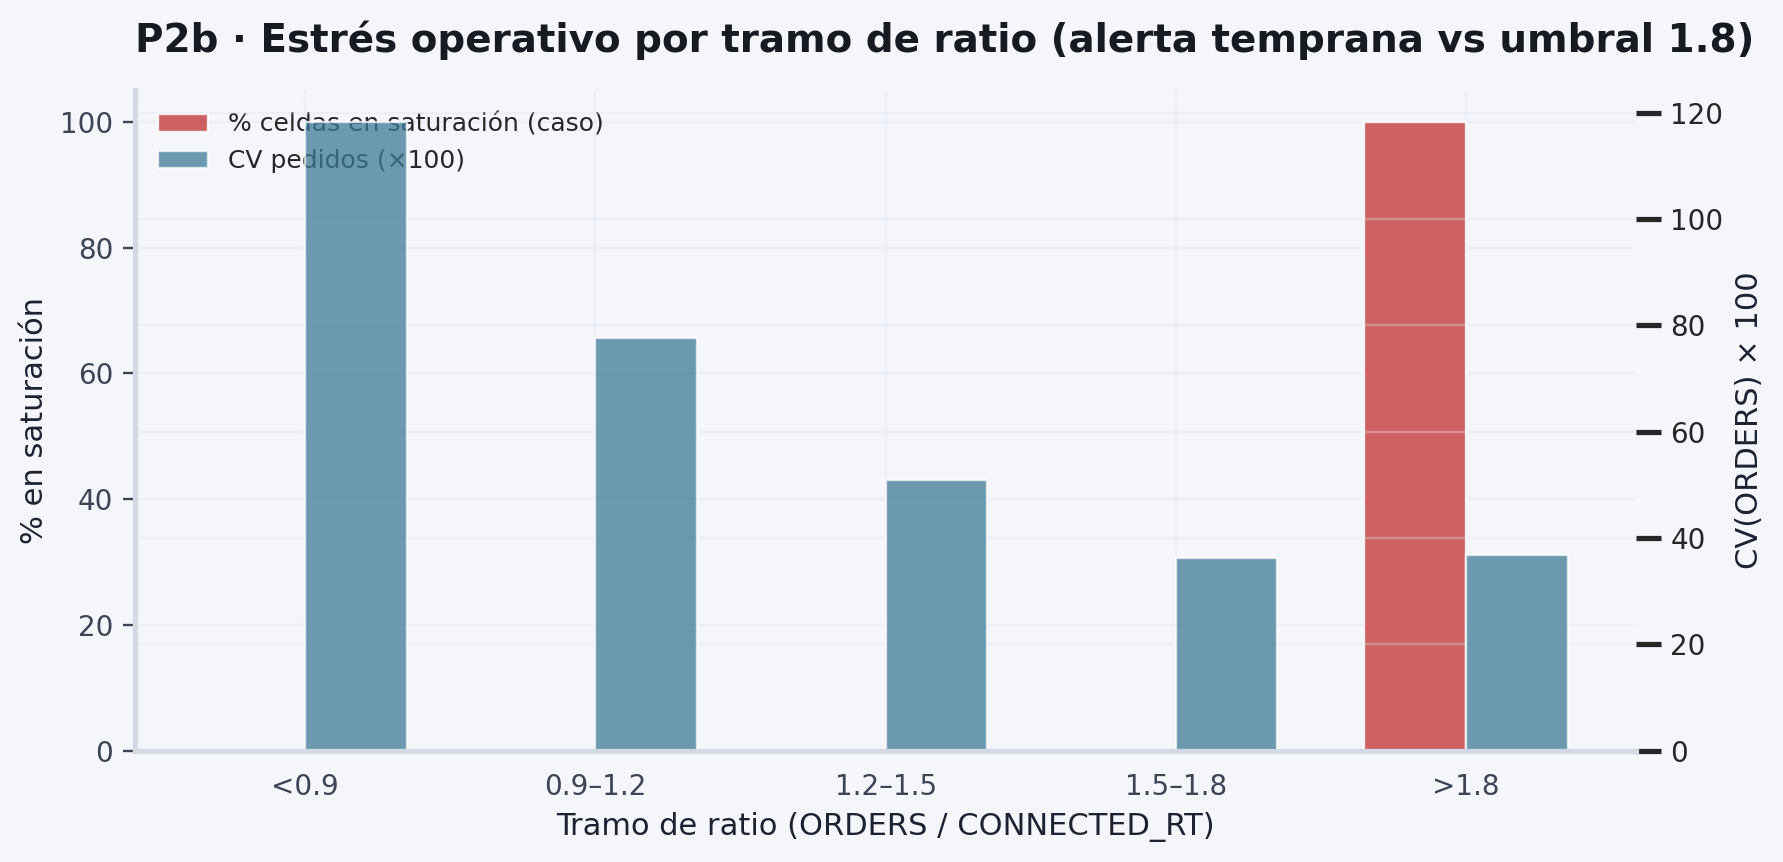
\includegraphics[width=\linewidth,height=0.70\textheight,keepaspectratio]{../modulo1_diagnostico/figures/p2_ratio_tramos_ops.png}
  \par
  \endgroup
  \begin{piegrafica}
  Las barras visualizan la misma lógica que la tabla: cómo cambia la fracción ya en saturación y la variabilidad de \texttt{ORDERS} al moverse el \texttt{ratio} por bandas.
  \end{piegrafica}
\end{frame}


\begin{frame}{P3 — Coef.\ precipitación por zona (MCO estratificado, 14 zonas)}
  \begingroup
  \scriptsize
  \centering
  \renewcommand{\arraystretch}{1.08}
  \begin{tabular}{@{}lr@{}}
    \toprule
    \textbf{Zona} & $\beta_{\text{precip}}$ \\
    \midrule
    Santiago            & $0{,}190569$ \\
    Carretera Nacional  & $0{,}131460$ \\
    Santa Catarina      & $0{,}103332$ \\
    MTY Apodaca Huinalá & $0{,}085885$ \\
    Independencia       & $0{,}073652$ \\
    San Pedro           & $0{,}068153$ \\
    Apodaca Centro      & $0{,}065663$ \\
    Escobedo            & $0{,}063273$ \\
    Centro              & $0{,}062092$ \\
    San Nicolás         & $0{,}059934$ \\
    La Fe               & $0{,}059660$ \\
    MTY Guadalupe       & $0{,}058108$ \\
    Cumbres Poniente    & $0{,}052032$ \\
    Mitras Centro       & $0{,}049596$ \\
    \bottomrule
  \end{tabular}
  \par
  \endgroup

  \begin{piegrafica}
  Por zona: \texttt{ratio} $\sim$ precip.\ + \texttt{C(HOUR)} + \texttt{C(dow)}. Orden por magnitud de $\beta$ (mismo criterio que el gráfico P3 del notebook).
  \end{piegrafica}
\end{frame}

\begin{frame}{P3 — Sensibilidad del \texttt{ratio} a la lluvia por zona}
  \begingroup
  \centering
  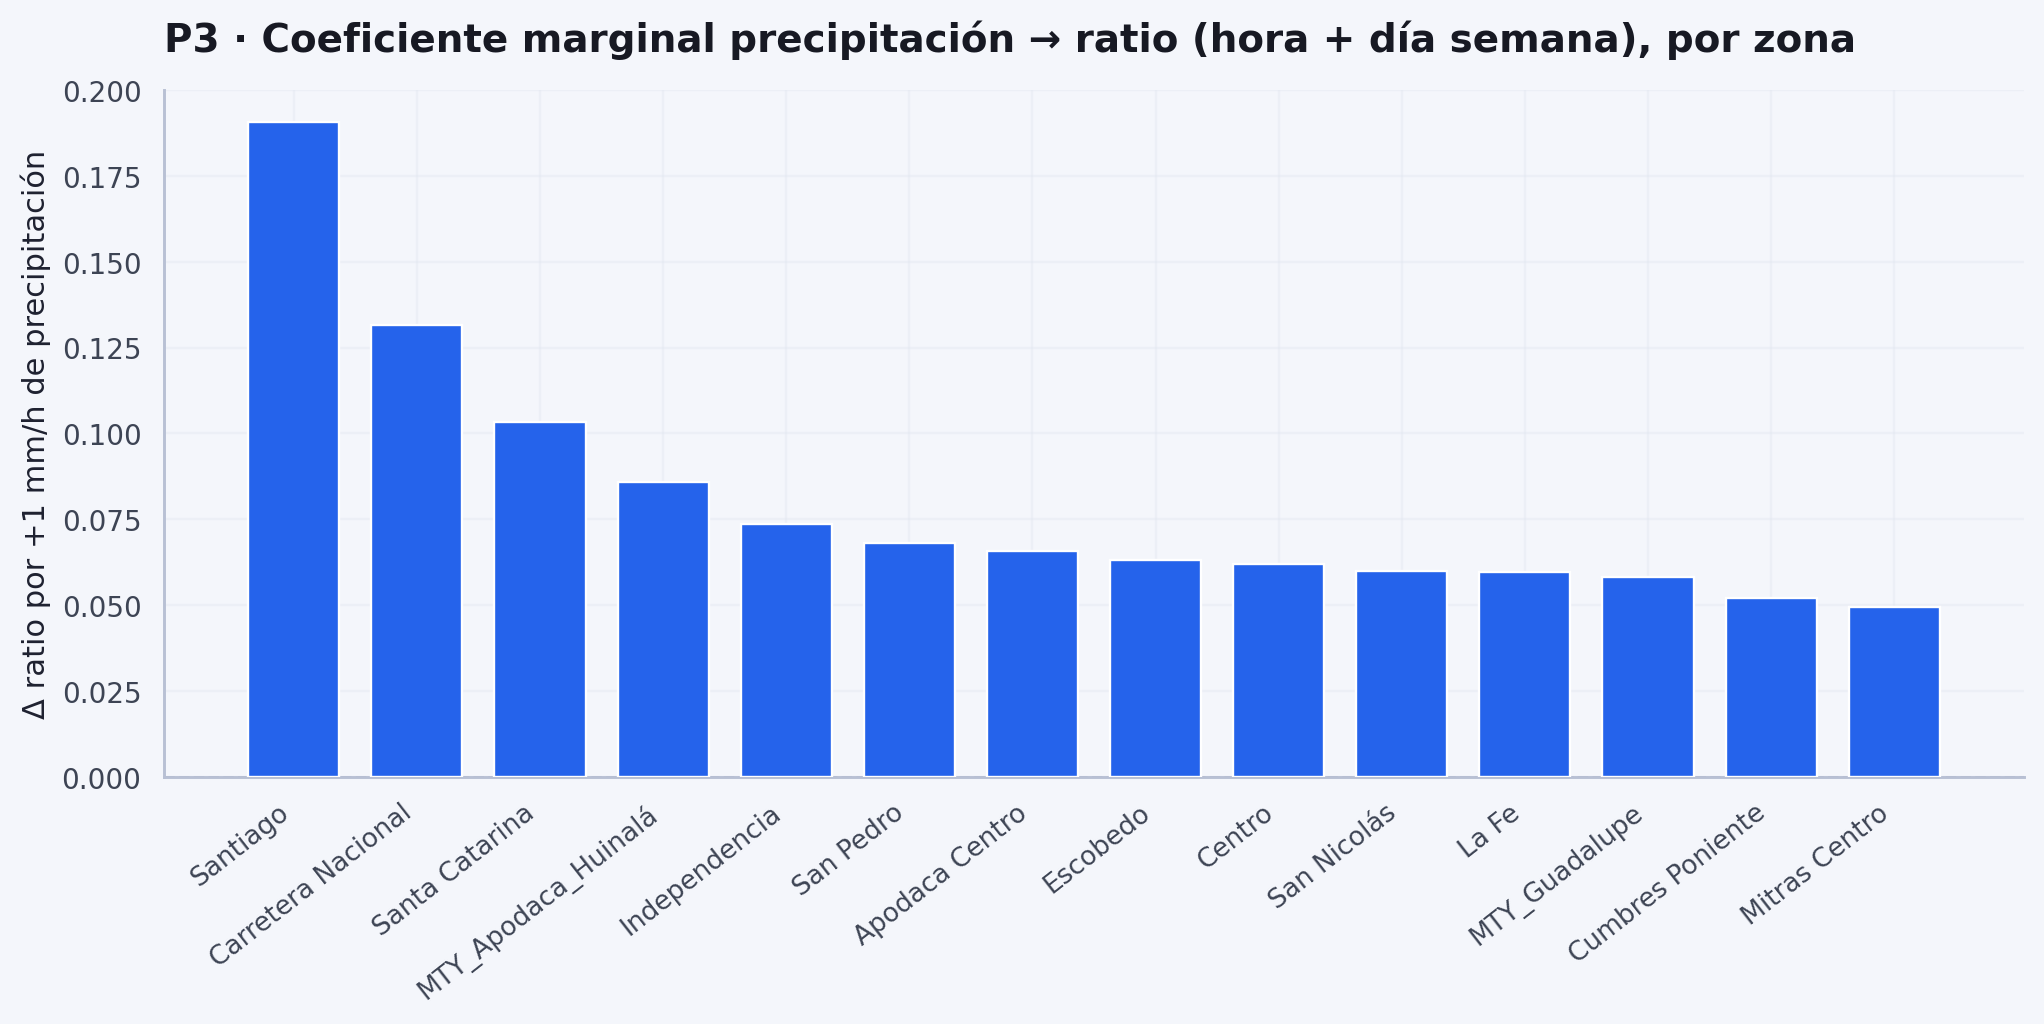
\includegraphics[width=\linewidth,height=0.70\textheight,keepaspectratio]{../modulo1_diagnostico/figures/p3_sensibilidad_zona.png}
  \par
  \endgroup
  \begin{piegrafica}
  El gráfico ordena territorios por magnitud del coeficiente marginal de precipitación (misma especificación dentro de cada \texttt{ZONE}).
  \end{piegrafica}
\end{frame}

\begin{frame}{P4 — Earnings diario vs fracción en saturación}
  \begingroup
  \centering
  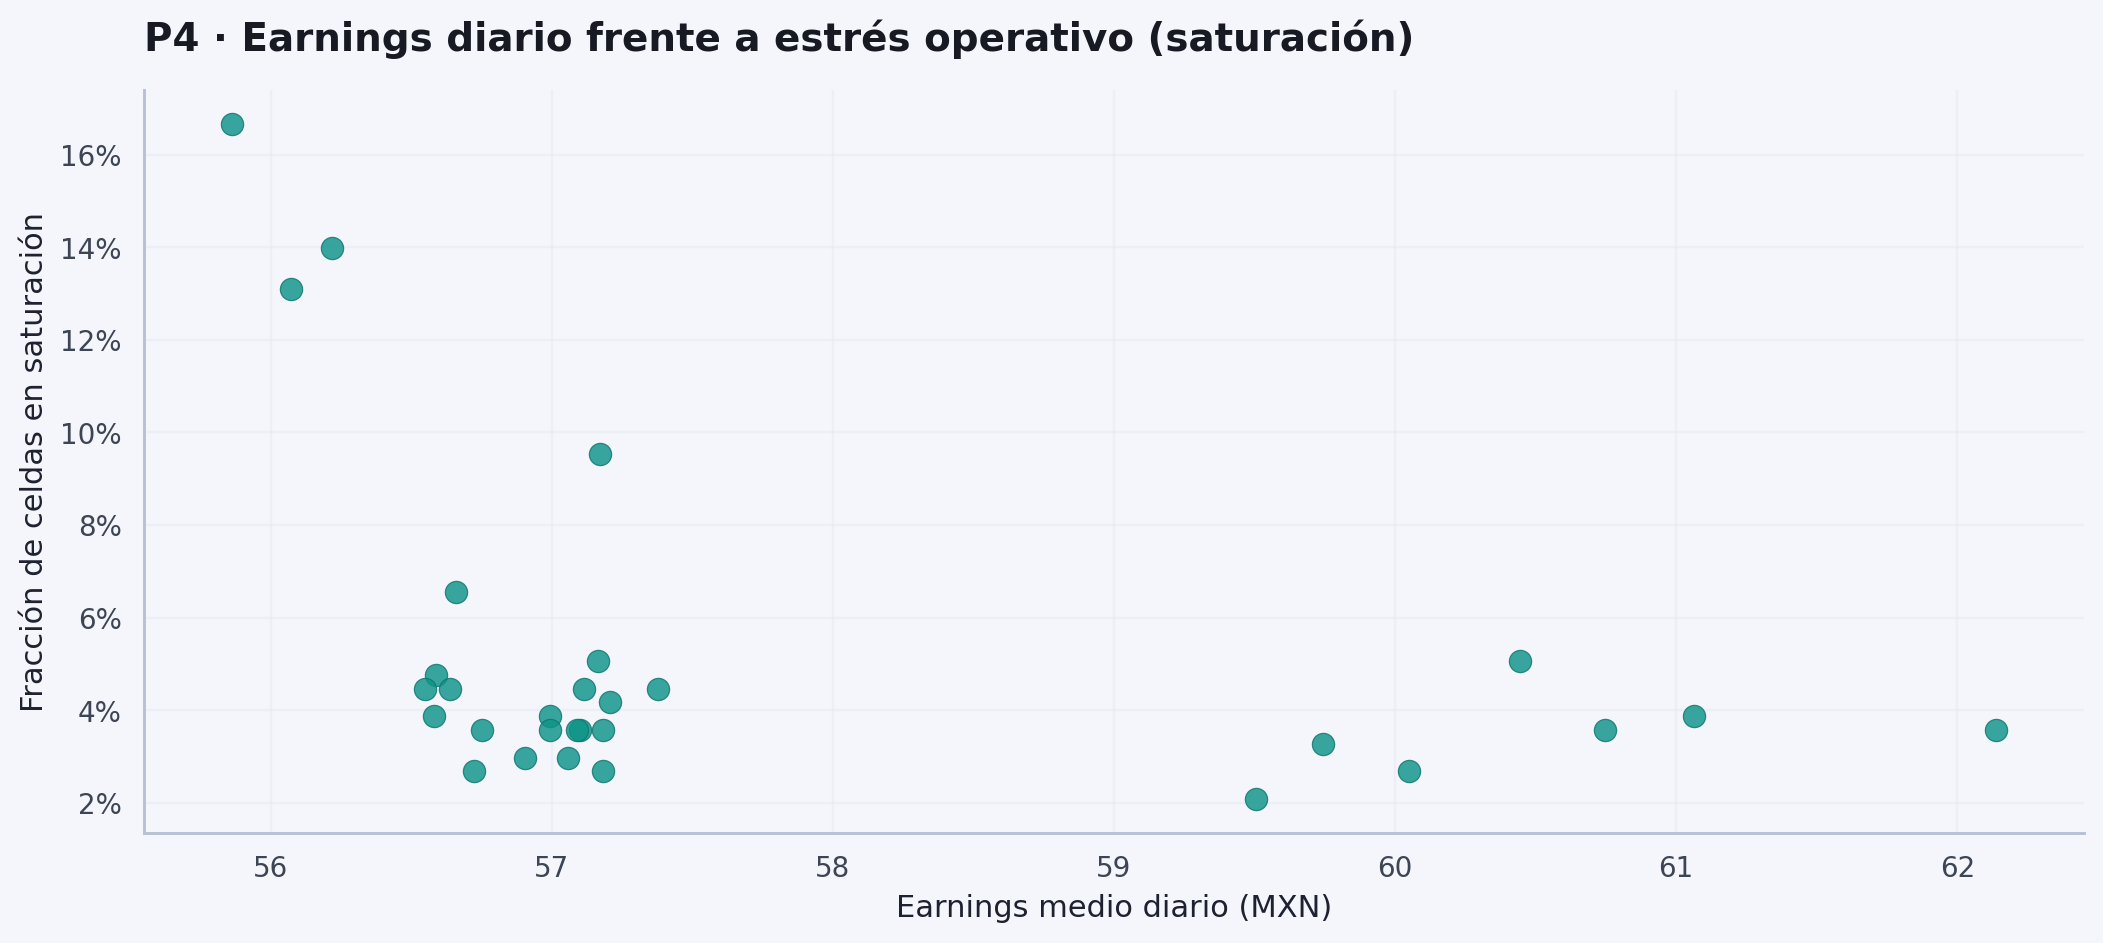
\includegraphics[width=\linewidth,height=0.70\textheight,keepaspectratio]{../modulo1_diagnostico/figures/p4_earnings_vs_estres.png}
  \par
  \endgroup
  \begin{piegrafica}
  Agrega por \textbf{día}: earnings medio frente a fracción de celdas en saturación. Sirve para ver días ``caros'' y estresados.

  Mezclar solo a nivel día puede confundir demanda e incentivos (véase GAP~4).
  \end{piegrafica}
\end{frame}

\begin{frame}{P4 — Top 10 días por \texttt{sat\_frac}}
  \begingroup
  \centering
  \scriptsize
  \renewcommand{\arraystretch}{1.05}
  \setlength{\tabcolsep}{3pt}
  \begin{tabular}{@{}lrrrr>{\raggedright\arraybackslash}p{0.42\linewidth}@{}}
    \toprule
    \textbf{Fecha} & \shortstack{earn.\\med.} & \texttt{sat\_frac} & \texttt{sobre\_frac} & \shortstack{\texttt{ratio}\\med.} & \textbf{A investigar (hip.\ ext.)} \\
    \midrule
    2024-03-28 & $55{,}86$ & $0{,}1667$ & $0{,}1994$ & $1{,}103$ &
      Placebo (Showcenter), The Vaccines (GNP). \\
    2024-03-08 & $56{,}22$ & $0{,}1399$ & $0{,}2173$ & $0{,}976$ &
      Neblina, Tour ``90s Pop'' (Arena), 8M \\
    2024-03-25 & $56{,}07$ & $0{,}1310$ & $0{,}2143$ & $0{,}896$ &
      Sin feriado\\
    2024-03-05 & $57{,}17$ & $0{,}0952$ & $0{,}2054$ & $0{,}980$ &
      Sin feriado. \\
    2024-03-27 & $56{,}66$ & $0{,}0655$ & $0{,}2143$ & $0{,}809$ &
      Sin eventos destacados. Sin feriado. \\
    2024-03-14 & $60{,}44$ & $0{,}0506$ & $0{,}2798$ & $0{,}746$ &
      Portugal. (Showcenter); Ana Bárbara (Arena).  \\
    2024-03-16 & $57{,}17$ & $0{,}0506$ & $0{,}2202$ & $0{,}800$ &
      Tucanes de Tijuana (Arena). \\
    2024-03-01 & $56{,}59$ & $0{,}0476$ & $0{,}1964$ & $0{,}831$ &
      Camilo Séptimo (Showcenter); Temerarios (Arena); \\
    2024-03-18 & $56{,}64$ & $0{,}0446$ & $0{,}2024$ & $0{,}814$ &
       Natalicio Benito Juárez, Laura Pausini (Arena). \\
    2024-03-26 & $56{,}55$ & $0{,}0446$ & $0{,}2173$ & $0{,}817$ &
      Sin feriado. \\
    \bottomrule
  \end{tabular}
  \par
  \endgroup
  \begin{piegraficafoot}
  Notebook: \textbf{p75 earn + estrés} solo 2024-03-14; \textbf{p75 earn + sobre-oferta} 2024-03-03, 07, 14, 22. Columna \emph{A investigar:} clima, conciertos/eventos y feriados (referencia externa; no está en el Excel del caso).
  \end{piegraficafoot}
\end{frame}


\begin{frame}{GAP 5 — \textit{Risk score} por zona (tabla completa, notebook)}
  \begingroup
  \centering
  \tiny
  \renewcommand{\arraystretch}{1.02}
  \begin{tabular}{@{}lrrrr@{}}
    \toprule
    \textbf{Zona} & \textbf{risk} & $\hat P_{\text{sat}}$ & sens.\ lluvia & demanda \\
    \midrule
    Santa Catarina      & $0{,}0832$ & $0{,}0528$ & $0{,}1033$ & $8{,}50$ \\
    Carretera Nacional  & $0{,}0616$ & $0{,}0597$ & $0{,}1315$ & $5{,}86$ \\
    San Nicolás         & $0{,}0507$ & $0{,}0625$ & $0{,}0599$ & $12{,}53$ \\
    Centro              & $0{,}0420$ & $0{,}0486$ & $0{,}0621$ & $16{,}11$ \\
    Independencia       & $0{,}0404$ & $0{,}0528$ & $0{,}0737$ & $8{,}84$ \\
    MTY Guadalupe       & $0{,}0341$ & $0{,}0611$ & $0{,}0581$ & $11{,}42$ \\
    Apodaca Centro      & $0{,}0292$ & $0{,}0514$ & $0{,}0657$ & $9{,}62$ \\
    San Pedro           & $0{,}0164$ & $0{,}0403$ & $0{,}0682$ & $13{,}67$ \\
    Escobedo            & $0{,}0139$ & $0{,}0500$ & $0{,}0633$ & $7{,}66$ \\
    Cumbres Poniente    & $0{,}0017$ & $0{,}0417$ & $0{,}0520$ & $9{,}96$ \\
    MTY Apodaca Huinalá & $0{,}0000$ & $0{,}0375$ & $0{,}0859$ & $4{,}48$ \\
    La Fe               & $0{,}0000$ & $0{,}0361$ & $0{,}0597$ & $7{,}64$ \\
    Mitras Centro       & $0{,}0000$ & $0{,}0556$ & $0{,}0496$ & $11{,}40$ \\
    Santiago            & $0{,}0000$ & $0{,}0625$ & $0{,}1906$ & $4{,}48$ \\
    \bottomrule
  \end{tabular}
  \par
  \endgroup

  \begin{piegrafica}
  $\text{risk} = \hat P(\text{sat}) \times \text{sensibilidad\_lluvia} \times \text{demanda}$ con factores min--max por columna en el panel (impreso en consola del notebook). Top~3: Santa Catarina, Carretera Nacional, San Nicolás.
  \end{piegrafica}
\end{frame}

\begin{frame}{GAP 5 — \textit{Risk score} por zona}
  \begingroup
  \centering
  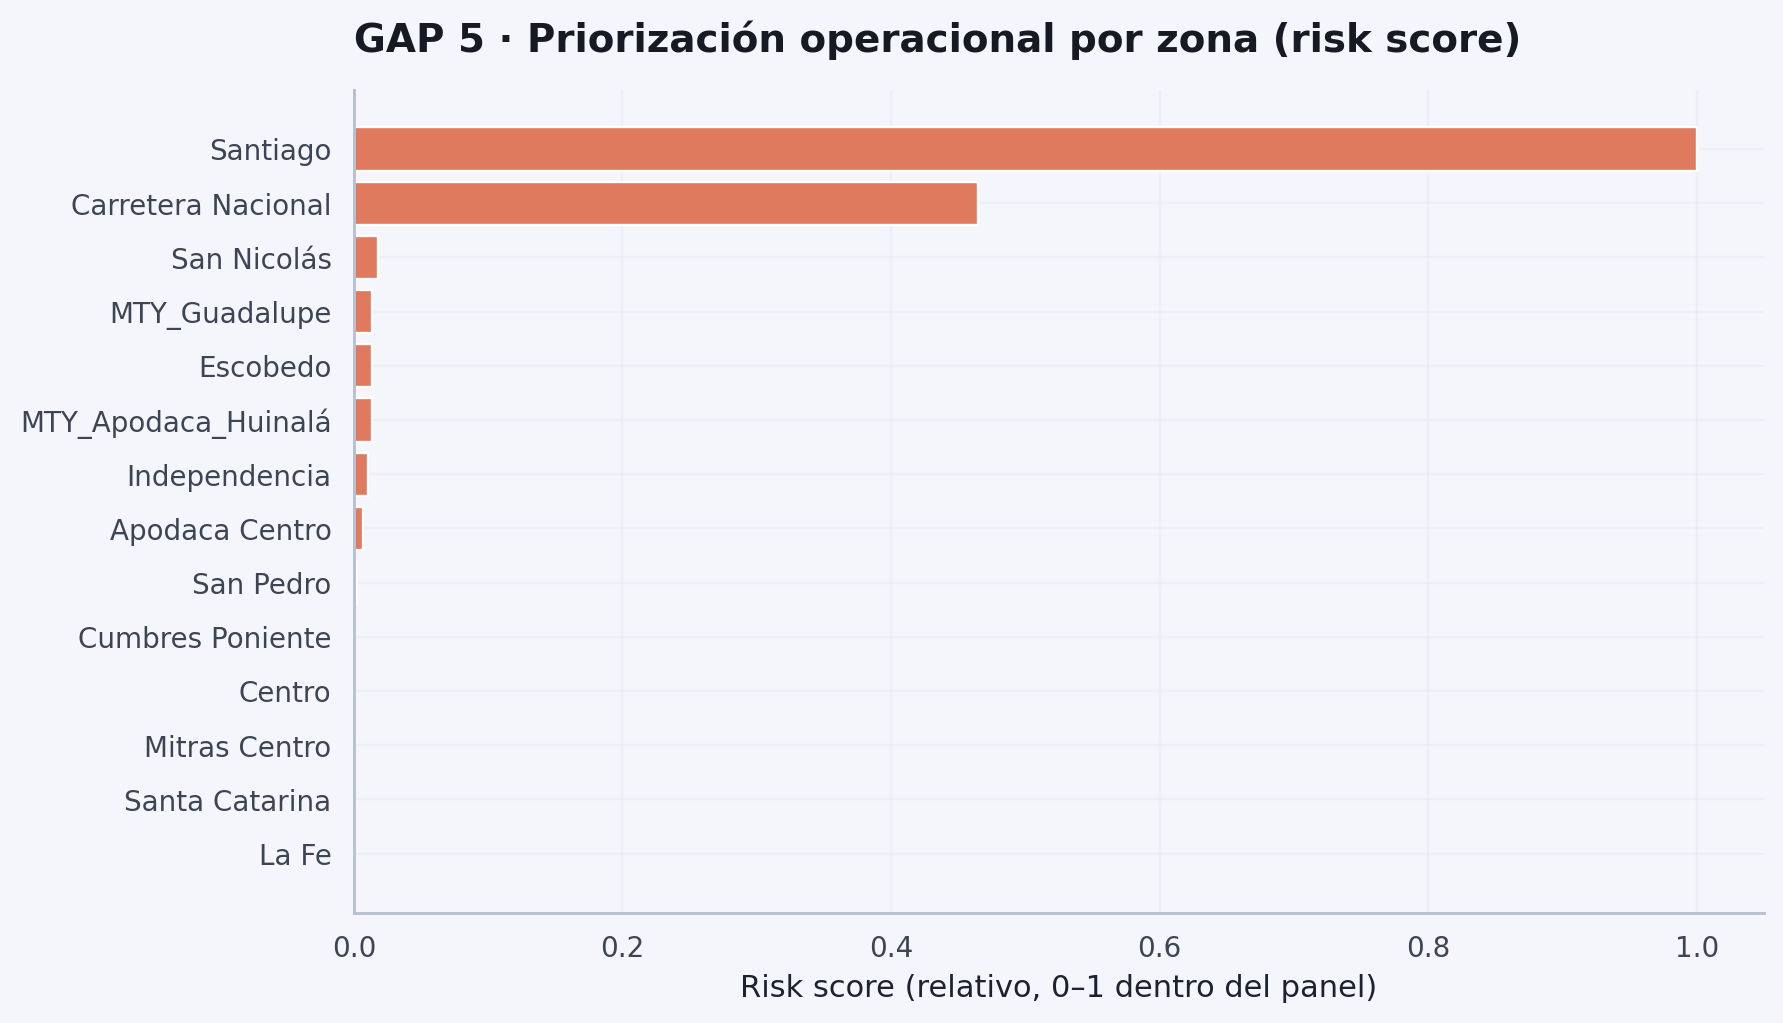
\includegraphics[width=\linewidth,height=0.70\textheight,keepaspectratio]{../modulo1_diagnostico/figures/gap5_risk_score_zonas.png}
  \par
  \endgroup
  \begin{piegrafica}
  Ranking visual coherente con la tabla; escala normalizada para comparar zonas en un solo gráfico.
  \end{piegrafica}
\end{frame}

\begin{frame}{Sensibilidad — mm/h para $\Delta\text{ratio}\approx 0{,}6$ (tabla)}
  \begingroup
  \centering
  \scriptsize
  \renewcommand{\arraystretch}{1.05}
  \begin{tabular}{@{}lrr@{}}
    \toprule
    \textbf{Zona} & $\beta_{\text{precip}}$ & mm/h ($\approx 0{,}6/\beta$) \\
    \midrule
    Santiago            & $0{,}1906$ & $3{,}15$ \\
    Carretera Nacional  & $0{,}1315$ & $4{,}56$ \\
    Santa Catarina      & $0{,}1033$ & $5{,}81$ \\
    MTY Apodaca Huinalá & $0{,}0859$ & $6{,}99$ \\
    Independencia       & $0{,}0737$ & $8{,}15$ \\
    San Pedro           & $0{,}0682$ & $8{,}80$ \\
    Apodaca Centro      & $0{,}0657$ & $9{,}14$ \\
    Escobedo            & $0{,}0633$ & $9{,}48$ \\
    Centro              & $0{,}0621$ & $9{,}66$ \\
    San Nicolás         & $0{,}0599$ & $10{,}01$ \\
    La Fe               & $0{,}0597$ & $10{,}06$ \\
    MTY Guadalupe       & $0{,}0581$ & $10{,}33$ \\
    Cumbres Poniente    & $0{,}0520$ & $11{,}53$ \\
    Mitras Centro       & $0{,}0496$ & $12{,}10$ \\
    \bottomrule
  \end{tabular}
  \par
  \endgroup
  \begin{piegraficafoot}
  Heurística del notebook: $\Delta\text{precip} \approx 0{,}6/\beta$ si $\beta>0$ (banda de \texttt{ratio} $1{,}2\to 1{,}8$). Lectura de orden de magnitud bajo linealidad local.
  \end{piegraficafoot}
\end{frame}

\begin{frame}{Sensibilidad — mm/h (gráfico)}
  \begingroup
  \centering
  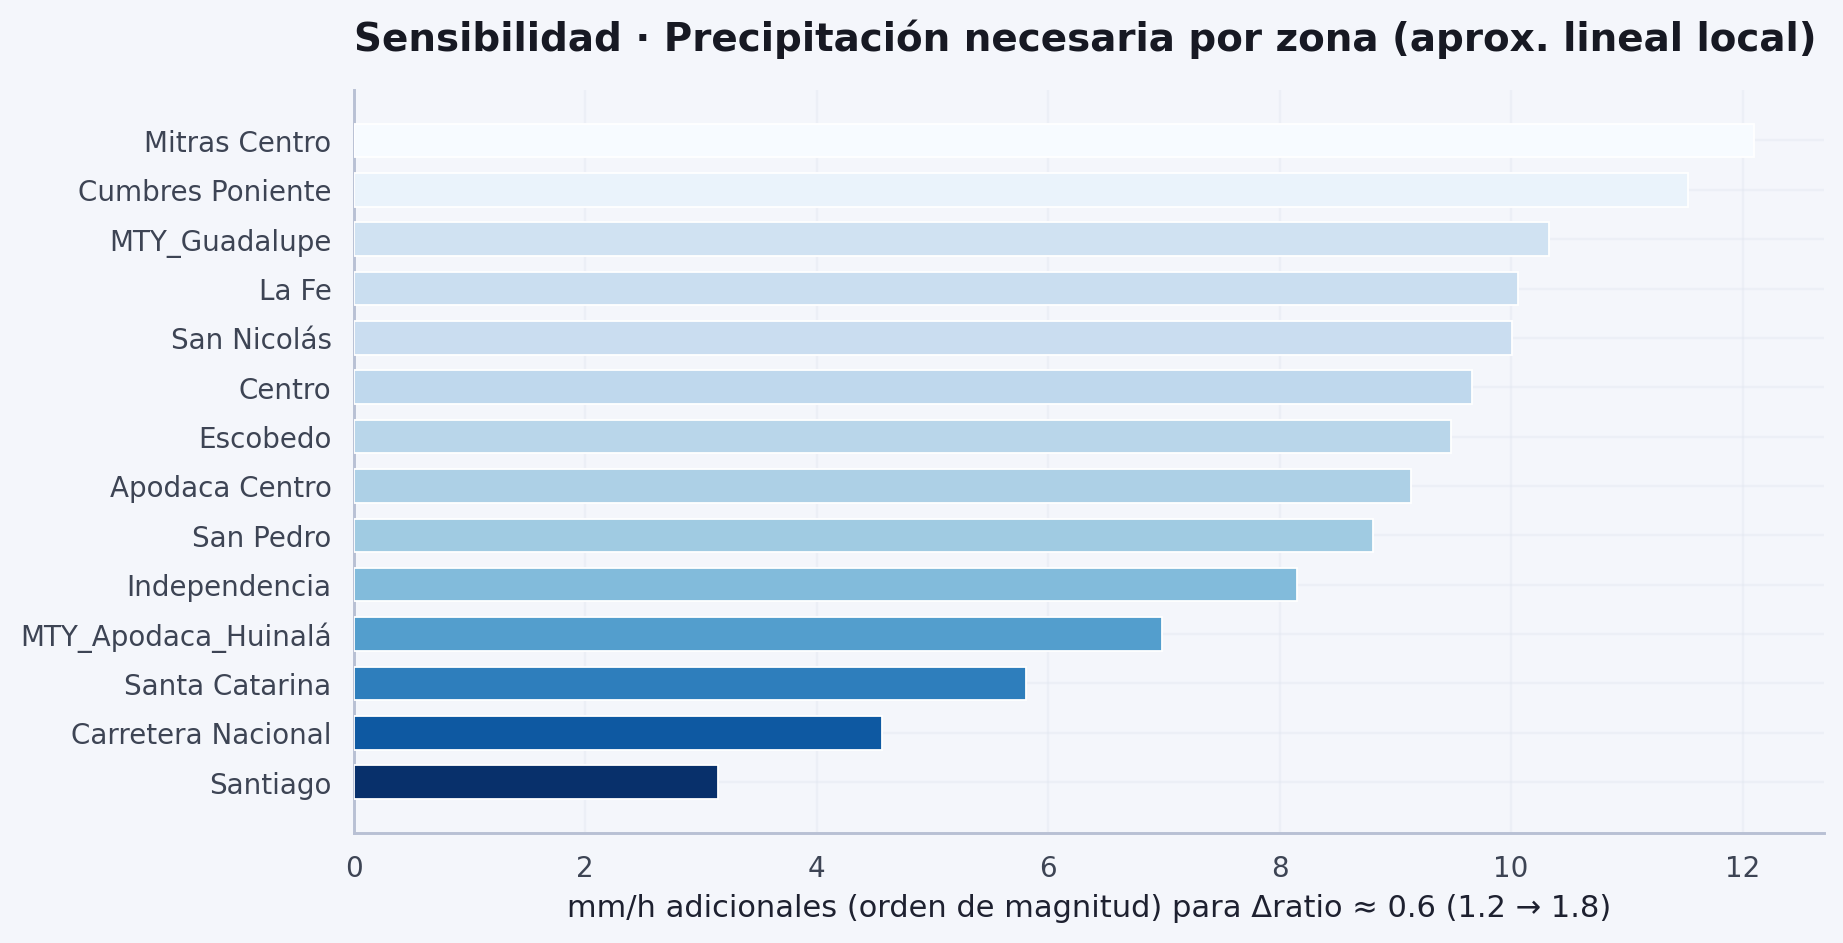
\includegraphics[width=\linewidth,height=0.70\textheight,keepaspectratio]{../modulo1_diagnostico/figures/p_sensitivity_mm_12_to_18.png}
  \par
  \endgroup
  \begin{piegrafica}
  Misma información que la tabla anterior en formato barras horizontales.
  \end{piegrafica}
\end{frame}



\begin{frame}{P5 — Spearman \texttt{EARNINGS} vs \texttt{ratio} (panel completo)}
  \begingroup
  \footnotesize
  \centering
  \renewcommand{\arraystretch}{1.2}
  \begin{tabular}{@{}lr@{}}
    \toprule
    \textbf{Contraste} & \textbf{Valor (notebook)} \\
    \midrule
    Spearman global ($n=10\,080$) & $\rho \approx 0{,}0761$ \\
    $p$-valor (dos colas) & $\approx 1{,}95\times 10^{-14}$ \\
    \bottomrule
  \end{tabular}
  \par
  \endgroup

  \begin{piegrafica}
  Correlación de \emph{rangos} (monótona, no lineal) entre tarifa y carga. Complementa Pearson y el MCO con interacción lluvia$\times$\texttt{EARNINGS} en la lámina siguiente.
  \end{piegrafica}
\end{frame}





% ---------------------------------------------------------------------------
\section{Insight clave: no es solo demanda}

\begin{frame}{Síntesis exploratoria (panel por zonas)}
  \small
  \textbf{Lectura exploratoria (Excel + notebook)}\\[0.6em]
  \begin{itemize}
    \item \textbf{Al parecer}, las zonas con perfil más \textbf{rural o periférico} concentran con mayor frecuencia \textbf{anomalías tipo saturación}: distribuciones más anchas y picos extremos (ratio muy alto en ciertas horas), coherentes con episodios de mucha demanda relativa frente a reparto disponible.
    \item Las zonas \textbf{urbanas y residenciales} tienden, en cambio, a que su \textbf{valor máximo habitual} quede \textbf{dentro del rango esperado} antes del umbral de saturación del panel: menos cola hacia valores extremos en el histórico mostrado.
  \end{itemize}
\end{frame}

\begin{frame}{Es contexto + tiempo}
  \begin{itemize}
    \item El estrés operativo no se reduce a ``hubo muchos pedidos'': importan \textbf{cuándo} (franja, festivo), \textbf{dónde} (zona) y \textbf{qué pasaba afuera} (lluvia) y con \textbf{qué incentivos} se operaba.
    \item El \texttt{ratio} resume desbalance oferta--demanda, pero su interpretación válida es \textbf{condicional} a hora y territorio.
    \item Por eso el caso calibra \textbf{por zona} y el motor mira \textbf{ventanas cortas} de clima, en lugar de una sola regla global.
  \end{itemize}
\end{frame}

% ---------------------------------------------------------------------------
\section{Acción: sistema de alertas y umbrales operativos}

\begin{frame}{Clima en vivo}
  \begin{itemize}
    \item \textbf{Open-Meteo:} pronóstico horario de lluvia, \textbf{sin API key} en el caso.
    \item Las unidades encajan con el Excel (mm por hora como intensidad).
    \item Zona horaria: \texttt{America/Monterrey}.
    \item Por defecto se miran unas \textbf{2 horas} hacia adelante (balance entre precisión y tiempo para reaccionar).
  \end{itemize}
\end{frame}


\begin{frame}{Qué hace el motor (pasos sencillos)}
  \small
  \begin{enumerate}
    \item Por zona: mira la lluvia máxima esperada frente al \textbf{umbral de esa zona}.
    \item Elige la zona \textbf{más preocupante} (mayor exceso sobre el umbral).
    \item Calcula cómo podría moverse el \textbf{ratio} con la lluvia prevista.
    \item Asigna \textbf{riesgo:} BAJO, MEDIO, ALTO o CRÍTICO.
    \item Propone \textbf{cuánto subir incentivos} y qué otras zonas vigilar.
  \end{enumerate}
\end{frame}

\begin{frame}{Para no ahogar al coordinador (debounce)}
  \begin{itemize}
    \item Se guarda un \textbf{estado por zona} (archivo local).
    \item No se repite el \textbf{mismo tipo de aviso} en poco tiempo (por defecto unos \textbf{45 minutos}), salvo que la situación \textbf{empeore de verdad} o suba mucho el \textbf{nivel de riesgo}.
    \item \textbf{Extra:} deduplicación del mismo ``evento'' de lluvia y, si se configura, tiempo mínimo entre alertas de \textbf{cualquier} zona (\texttt{ALERT\_GLOBAL\_MIN\_INTERVAL\_SEC}).
  \end{itemize}
\end{frame}

\begin{frame}{Cómo probar el motor solo}
  \texttt{modulo2\_motor\_alertas/run\_alert\_engine.py}
  \vspace{0.5em}
  \begin{itemize}
    \item \texttt{python run\_alert\_engine.py} — usa clima real, resultado en consola.
    \item \texttt{python run\_alert\_engine.py --demo} — simula lluvia fuerte en Santiago sin internet.
    \item \texttt{python run\_alert\_engine.py --recalibrate} — vuelve a armar \texttt{calibration.json} desde el Excel y ejecuta.
  \end{itemize}
  \vspace{0.3em}
  \small Reglas explicadas en lenguaje llano: \texttt{motor\_reglas/motor\_reglas.tex} $\rightarrow$ PDF.
\end{frame}

\begin{frame}{Módulo 3 — Telegram: mismo motor, texto para humanos}
  \begin{itemize}
    \item Mismo clima y \textbf{mismo motor} que el M2.
    \item El programa arma un \textbf{resumen en JSON} (zona, riesgo, números); el modelo de lenguaje solo \textbf{redacta} el mensaje.
    \item Puede usarse \textbf{Ollama} en local o \textbf{OpenAI}; con OpenAI, por defecto entra \textbf{LangChain}. Si el modelo falla, hay \textbf{texto fijo} con los mismos datos.
    \item El envío es con \textbf{python-telegram-bot}.
  \end{itemize}
\end{frame}

\begin{frame}{Qué debe verse en el mensaje (unos 10 segundos)}
  \begin{itemize}
    \item Zona y \textbf{qué tan grave} es.
    \item Qué lluvia se espera y en qué ventana.
    \item Una frase de \textbf{contexto histórico} (guiada por el sistema).
    \item \textbf{Acción clara:} subir pagos de X a Y pesos en Z minutos.
    \item Otras \textbf{zonas a vigilar}.
  \end{itemize}
\end{frame}


\begin{frame}{Dos tiempos distintos}
  \begin{itemize}
    \item \textbf{Cada cuánto se mira el clima} (monitor): p.\,ej. cada 10 min.
    \item \textbf{Cada cuánto se puede repetir} un aviso parecido en la misma zona: p.\,ej. $\sim$45 min.
    \item Si el \textbf{riesgo sube de nivel}, puede avisarse antes aunque no haya pasado el tiempo largo.
  \end{itemize}
\end{frame}


% ---------------------------------------------------------------------------
\section{Extensión futura}

\begin{frame}{Próximos pasos posibles}
  \begin{itemize}
    \item \textbf{ML predictivo:} modelo de \texttt{ratio} o de probabilidad de saturación en ventanas cortas (features: lluvia prevista, hora, zona, histórico reciente), en paralelo a reglas interpretables.
    \item \textbf{Optimización logística:} acoplar sugerencias de incentivos con restricciones reales de flota, costo marginal y políticas comerciales; cerrar el ciclo con experimentación controlada.
    \item \textbf{Más señales:} demanda prevista, eventos locales, integración con despacho en vivo.
  \end{itemize}
\end{frame}



\begin{frame}{}
  \centering
  {\Huge Gracias}

\end{frame}

\end{document}
